\newpage
\section{Virtualisation embarquée}
\subsection{Test de l'environnement EmbeddedXEN}
Tous les fichiers relatifs à l'environnement de virtualisation EmbeddedXEN, à l'exception du système
de fichiers (rootfs) préparé précédemment, se trouvent dans le répertoire embeddedxen situé dans votre
workspace.\\\\
\textbf{a) Donnée: }Le paramètre ex peut être utilisé avec le script deploy pour le déploiement des fichiers dans le rootfs
utilisé avec EmbeddedXEN, comme suit :
\begin{lstlisting}
$ ./deploy ex
\end{lstlisting}
Déployez les fichiers dans le nouveau \textit{rootfs}\\\\
\textbf{Travail réalisé: }Cette commande déploie les fichiers dans le rootfs de l'environnement de virtualisation.
\begin{lstlisting}
$ cd ~/seee_student/
$ ./deploy ex
Deploying into EmbeddedXEN rootfs ...
Mounting filesystem/reptar4-sdcard.img...
[sudo] password for redsuser: 
SD card partitions mounted in 'boot_tmp' and 'filesystem_tmp' directories
Unmounting SD card image...
Synchronizing .img file
Unmounting 'boot_tmp' and 'filesystem_tmp'...
Done !
$ 
\end{lstlisting}
\textbf{Remarque: }Il est très important de ne pas avoir de message d'erreur lors de l'exécution de cette commande. Si un message comme ci-dessous est observé, cela indique que l'image contenant le rootfs est corrompue. L'unique solution pour résoudre ce problème est de la télécharger à nouveau.
\begin{lstlisting}
mount: wrong fs type, bad option, bad superblock on /dev/loop1,
missing codepage or helper program, or other error
In some cases useful info is found in syslog - try
dmesg | tail  or so
\end{lstlisting}
\textbf{b) Donnée: }Démarrez le système en lançant le script ./stex.\\\\
\textbf{Travail réalisé: }Avec ce script on arrive dans l'U-boot et l'environnement graphique de la carte Reptar est lancé.
\begin{lstlisting}
$ ./stex
...
Reptar # 
\end{lstlisting}
\textbf{c) Donnée: }Vous pouvez observer le démarrage de l'hyperviseur, suivi du premier OS invité (Dom0), puis du
second OS invité (DomU). Les messages seront "mélangés" par la suite car les deux OS accèderont
simultanément à l'UART de la console. La commutation de la console entre Dom0 et DomU, puis
entre DomU et la console de l'hyperviseur, puis entre cette dernière et Dom0 de nouveau, s'effectue
à l'aide de trois combinaisons Ctrl-A successives (3 x Ctrl-A). Connectez-vous dans les deux
domaines (login et mot de passe : root).\\\\
\textbf{Travail réalisé: }Pour que l'hyperviseur démarre, il faut commencer par booter. On voit ensuite le démarrage de DOM-U, DOM-0 et l'hyperviseur XEN. À la fin du boot, on arrive dans le DOM-U où il faut entrer un mot de passe. Avec trois Ctrl-A, on peut commuter la console et passer dans DOM-0. La capture ci-dessous présente les tests effectués. 
\begin{lstlisting}
Reptar # boot
...
*** Welcome on REPTAR (HEIG-VD/REDS): use root/root to log in ***
reptar login: [DOM-U] EXT2-fs (xvda1): warning: mounting unchecked fs, running e2fsck is recommended
[DOM-U] VFS: Mounted root (ext2 filesystem) on device 202:1.
[DOM-U] Freeing init memory: 88K
[DOM-U] ### HELLO FROM domU !!
...

[DOM-U] *** Welcome on REPTAR (HEIG-VD/REDS): use root/root to log in ***
reptar login: root
Password: 
# ls
Settings  config    qtrun

# *** Serial input -> DOMU (type 'CTRL-a' three times to switch input to Xen).
[DOM-0] <4>*** Serial input -> Xen (type 'CTRL-a' three times to switch input to DOM0).
[DOM-0] <4>*** Serial input -> DOM0 (type 'CTRL-a' three times to switch input to DOMU).
# ls
Settings  config    qtrun

# [DOM-0] <4>*** Serial input -> DOMU (type 'CTRL-a' three times to switch input to Xen).
[DOM-U] 
[DOM-U] *** Welcome on REPTAR (HEIG-VD/REDS): use root/root to log in ***
reptar login: 
\end{lstlisting}
\subsection{Déploiement du driver sp6 dans Dom0}
Dans cette étape, vous allez déployer votre driver sp6 dans Dom0. Pour cela, il faut d'abord le
recompiler pour le noyau correspondant à ce domaine.\\\\
\textbf{a) Donnée: }Modifiez le Makefile dans le répertoire drivers afin que la compilation du module s'effectue avec
le noyau linux-3.0-reptar-dom0 présent dans embeddedxen, et non plus avec le noyau linux-3.0-
reptar\\\\
\textbf{Emplacement du code: }\textit{/virtualisation\_part2/Makefile}\\\\
\textbf{Travail réalisé: }La ligne suivante a été changée dans le Makefile pour compiler avec le noyau dom0.
\begin{lstlisting}
#KDIR	= ../linux-3.0-reptar
KDIR	= ../embeddedxen/linux-3.0-reptar-dom0
\end{lstlisting}
\textbf{b) Donnée: }Compilez votre module.\\\\
\textbf{Travail réalisé: }
\begin{lstlisting}
$ cd ~/seee_student/drivers/
$ make clean all
$ make
make -C ../embeddedxen/linux-3.0-reptar-dom0 
...
CC      /home/redsuser/seee_student/drivers/sp6.mod.o
LD [M]  /home/redsuser/seee_student/drivers/sp6.ko
make[1]: Leaving directory `/home/redsuser/seee_student/embeddedxen/linux-3.0-reptar-dom0'
$ 
\end{lstlisting}
\textbf{c) Donnée: }Déployez votre module dans le rootfs de Dom0 avec ./deploy ex .\\\\
\textbf{Travail réalisé: }
\begin{lstlisting}
$ cd ~/seee_student/
$ ./deploy ex
Deploying into EmbeddedXEN rootfs ...
Mounting filesystem/reptar4-sdcard.img...
[sudo] password for redsuser: 
SD card partitions mounted in 'boot_tmp' and 'filesystem_tmp' directories
Unmounting SD card image...
Synchronizing .img file
Unmounting 'boot_tmp' and 'filesystem_tmp'...
Done !
$
\end{lstlisting}
\textbf{d) Donnée: }Démarrez QEMU\\\\
\textbf{Travail réalisé: }Avec la commande \textit{./stex}, puis boot pour démarrer l'hyperviseur.
\begin{lstlisting}
$ cd ~/seee_student/
$ ./stex
...
Reptar # boot
...
\end{lstlisting}
\textbf{e) Donnée: }Dans Dom0, restez dans le répertoire /root, chargez le module puis lancez l'application ./qtrun :
\begin{lstlisting}
# cd
# insmod /sp6.ko
# ./qtrun
\end{lstlisting}
\textbf{Travail réalisé: }On voit ci-dessous que le driver est correctement inséré. lorsque l'on lance qtrun, cela va ouvrir QTextEdit dans la fenête Qemu que nous n'avions pas utilisée jusqu'ici. Cette fenêtre est une représentation graphique de l'écran tactile de la carte Reptar.
\begin{lstlisting}
# *** Serial input -> DOMU (type 'CTRL-a' three times to switch input to Xen).
[DOM-0] <4>*** Serial input -> Xen (type 'CTRL-a' three times to switch input to DOM0).
[DOM-0] <4>*** Serial input -> DOM0 (type 'CTRL-a' three times to switch input to DOMU).
# cd
# insmod /sp6.ko 
[DOM-0] <4>reptar_sp6: module starting...
[DOM-0] <4>Probing FPGA driver (device: fpga)
[DOM-0] <7>Registered led device: sp6_led0
[DOM-0] <7>Registered led device: sp6_led1
[DOM-0] <7>Registered led device: sp6_led2
[DOM-0] <7>Registered led device: sp6_led3
[DOM-0] <7>Registered led device: sp6_led4
[DOM-0] <7>Registered led device: sp6_led5
[DOM-0] <4>btns_reg address : 0xc5c18012
[DOM-0] <4>irq_reg address : 0xc5c1a018
sp6_read: Button irq status read 0x0 (button value 0x1)
sp6_write: Button irq status write 0x80
Enable IRQ
[DOM-0] <6>input: reptar_sp6_buttons as /devices/platform/fpga/reptar_sp6_buttons/input/input1
[DOM-0] <4>reptar_sp6: done.
# ./qtrun
\end{lstlisting}
Voici ci-dessous le contenu du script qtrun. On voit qu'il exécute les mêmes commandes que lorsque l'on a testé le driver des boutons dans le précédent labo. Les entrées sont liées au fichier /dev/input/event1.
\begin{lstlisting}
cd /usr/share/qt/demos/textedit
export QWS_KEYBOARD="LinuxInput:/dev/input/event1"
./textedit -qws
\end{lstlisting}
On peut tester que notre driver contrôlant les boutons fonctionne correctement en regardant la fenêtre QTextEdit. Lorsque l'on presse les boutons, on arrive a faire des espaces dans le texte, déplacer le curseur, mettre en gras...etc. On a donc un driver qui fonctionne dans Dom0 avec accès au matériel émulé.
\begin{figure}[H]
	\begin{center}
		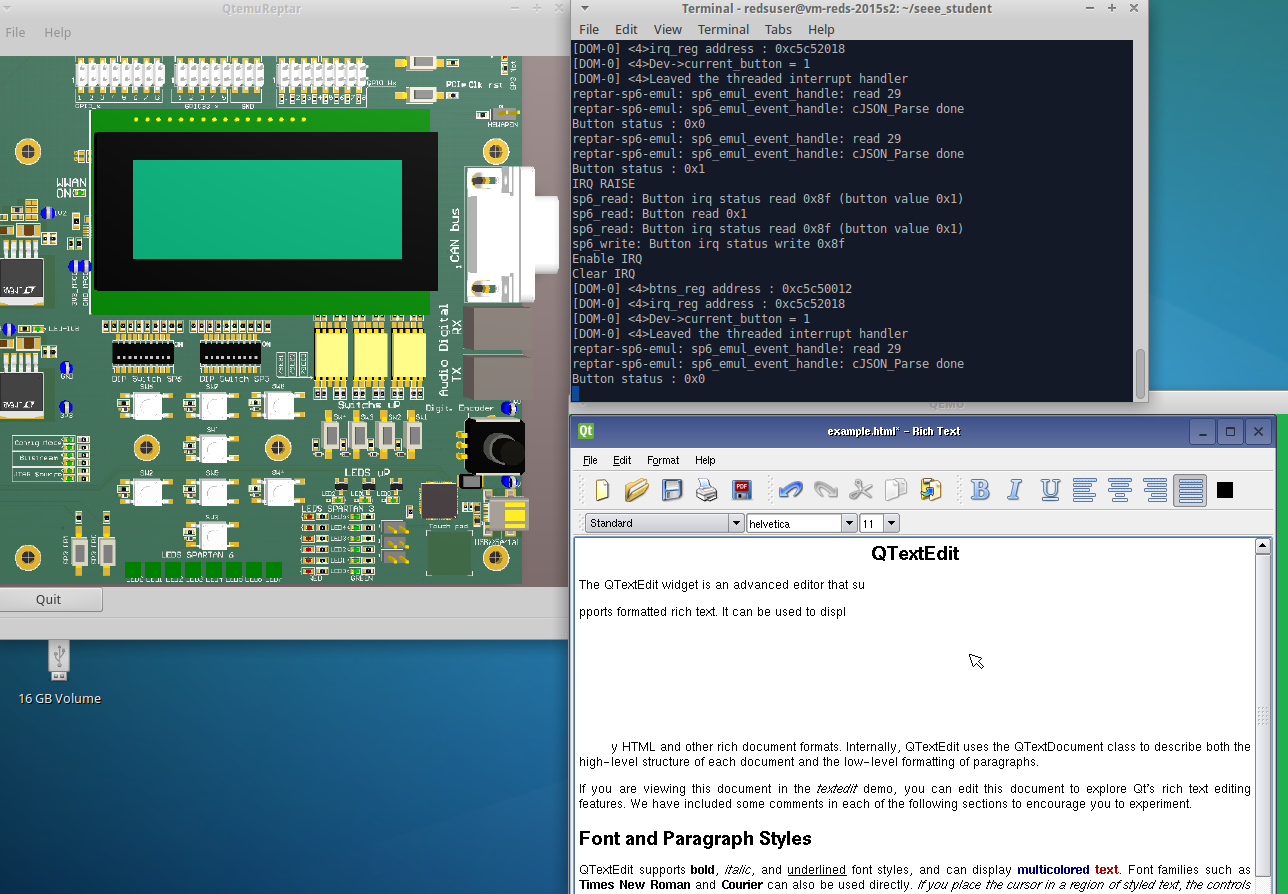
\includegraphics[width=16cm]{img/dom0.png}
		\caption{Exécution de Qtrun dans Dom0}
		\label{qtrun}
	\end{center}
\end{figure}
\subsection{Interaction entre Dom0 et DomU sur l'interface input para-virtualisé}
Dom0 peut accéder directement aux périphériques et les piloter, mais DomU ne le peut pas. Ainsi, nous
avons besoin de créer une interface virtuelle dans DomU pour lui permettre d’accéder aux ressources
du périphérique souhaité, en assurant une bonne coordination des accès. Les drivers sont découpés en
deux parties : le backend dans Dom0 et le frontend dans DomU.\\\\
Lors de cet exercice, nous allons permettre à l’application Qt dans DomU de récupérer les événements
input (input events) provenant de la FPGA.\\\\
\textbf{a) Donnée: }Identifiez les différents blocs qui interviennent lors de la propagation de l’input event depuis la
FPGA vers DomU. Etablissez un schéma faisant intervenir différents blocs : le backend input, le
driver FPGA développé par vos soins, le frontend input, les input subsystems de Dom0 et DomU…
(Vous trouverez le backend dans linux-3.0-reptar-dom0/drivers/input/xen-kbdback et le frontend
dans linux-3.4.6-domU/drivers/input/misc/xen-kbdfront.c ).\\\\
\textbf{Travail réalisé: }Voici une représentation de la propagation d'un événement input du matériel vers DomU avec les deux espaces, utilisateur et noyau.
\begin{figure}[H]
	\begin{center}
		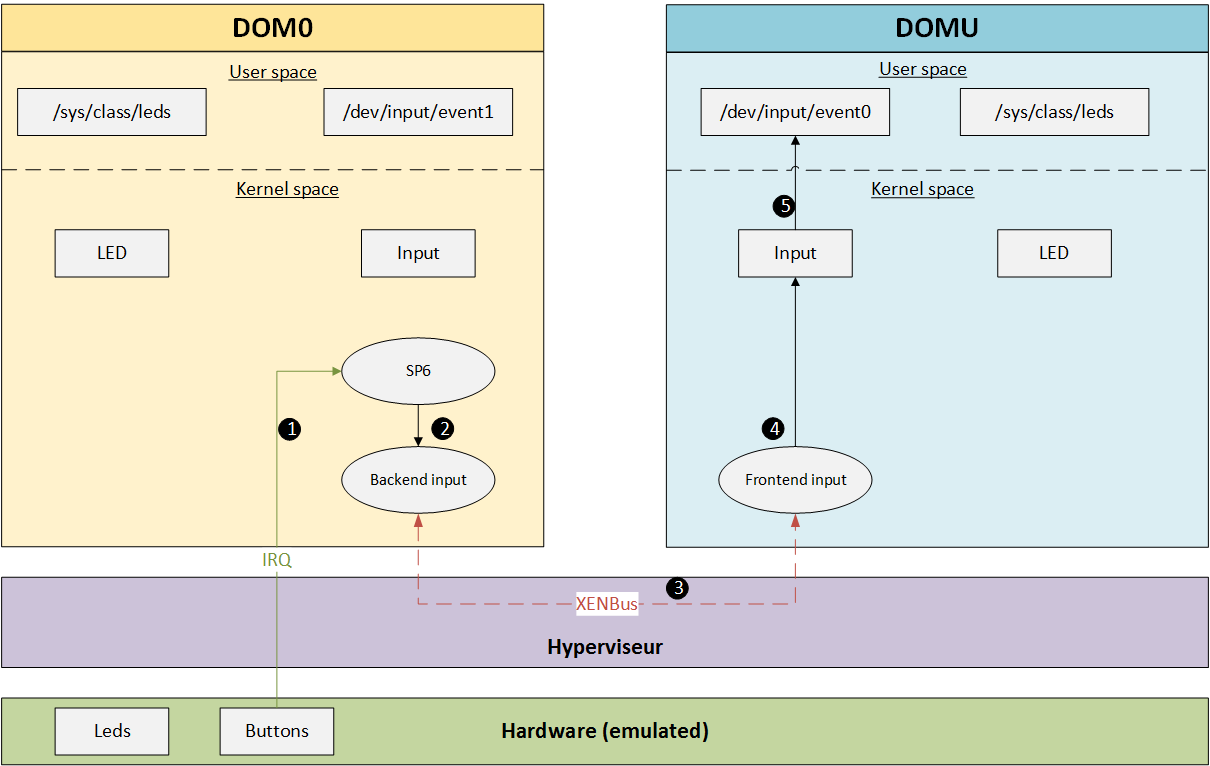
\includegraphics[width=17cm]{img/virt1.png}
		\caption{Propagation de l'input event jusqu'à DomU}
		\label{virt1}
	\end{center}
\end{figure}
Étapes de la propagation:
\begin{enumerate}
	\item L'interruption matérielle est interceptée par notre driver SP6 qui est présent uniquement dans Dom0
	\item Si le focus est placé sur DomU, l'événement est propagé au driver backend input. Notre driver SP6 s'est préalablement enregistré auprès du backend.
	\item L'hyperviseur transmet l'information au travers du XenBus
	\item Le driver frontend dans DomU reçoit l'input event. Il le transmet ensuite au module input de DomU
	\item L'événement se retrouve en espace utilisateur dans le fichier \textit{/dev/input/event0}\\
\end{enumerate}
\textbf{b) Donnée: }Modifiez votre driver afin que celui-ci s'enregistre auprès du backend input à l'aide de la fonction
xenvkbd\_inputdev\_register( ) (quelques indications sont fournies ci-après).\\\\
\textbf{Emplacement du code: }\textit{/virtualisation\_part3/reptar\_sp6\_buttons.c}\\\\
\textbf{Travail réalisé: }\\Le fichier \textit{reptar\_sp6\_buttons.c} pour s'enregistrer auprès du backend input.
\begin{lstlisting}
/*Register to backend */
xenvkbd_inputdev_register(&input, GPIOKEY);
\end{lstlisting}
Le focus change entre DomU et Dom0 lors de l'appui sur les deux boutons droite/gauche du haut. Dans la donnée, il manquait la méthode \textit{xenfb\_set\_focus} qui permet de changer le focus. La méthode \textit{omapfb\_xen\_switch\_domain} permet de rediriger le framebuffer.
\begin{lstlisting}
if(dev->current_button == 0x80)
{
	omapfb_xen_switch_domain(1);
	xenfb_set_focus(1);
}
else if(dev->current_button == 0x20)
{
	omapfb_xen_switch_domain(0);
	xenfb_set_focus(0);
}
\end{lstlisting}
Voici une capture du test réalisé. Il faut insérer le driver Sp6 dans Dom0 et uniquement à cet endroit. On peut ensuite lancer l'application \textit{qtrun}. Pour démarrer le programme dans DomU, il suffit de faire trois fois Ctrl-A, \textit{qtrun} est également disponible.
\begin{lstlisting}
[DOM-U] *** Welcome on REPTAR (HEIG-VD/REDS): use root/root to log in ***
reptar login: root
Password: 
# *** Serial input -> DOMU (type 'CTRL-a' three times to switch input to Xen).
[DOM-0] <4>*** Serial input -> Xen (type 'CTRL-a' three times to switch input to DOM0).
[DOM-0] <4>*** Serial input -> DOM0 (type 'CTRL-a' three times to switch input to DOMU).

# cd
# insmod /sp6.ko 
[DOM-0] <4>reptar_sp6: module starting...
[DOM-0] <4>Probing FPGA driver (device: fpga)
[DOM-0] <7>Registered led device: sp6_led0
[DOM-0] <7>Registered led device: sp6_led1
[DOM-0] <7>Registered led device: sp6_led2
[DOM-0] <7>Registered led device: sp6_led3
[DOM-0] <7>Registered led device: sp6_led4
[DOM-0] <7>Registered led device: sp6_led5
[DOM-0] <4>btns_reg address : 0xc5c4c012
[DOM-0] <4>irq_reg address : 0xc5c4e018
sp6_read: Button irq status read 0x0 (button value 0x1)
sp6_write: Button irq status write 0x80
Enable IRQ
[DOM-0] <6>input: reptar_sp6_buttons as /devices/platform/fpga/reptar_sp6_buttons/input/input1
[DOM-0] <4>reptar_sp6: done.
# ./qtrun
[DOM-0] <4>*** Serial input -> DOMU (type 'CTRL-a' three times to switch input to Xen).
[DOM-U] *** Welcome on REPTAR (HEIG-VD/REDS): use root/root to log in ***
[DOM-U] reptar login: root 
[DOM-U] Password: 
# ./qtrun 
\end{lstlisting}
Voici deux captures d'écran prouvant le bon fonctionnement de la transmission de l'input event dans les deux domaines. En appuyant sur les boutons indiqués d'une flèche rouge, on passe d'un dommaine à l'autre, avec les autres boutons, on agit sur le texte de l'application. On voit ci-dessous que les écrans ne sont pas les mêmes entre les deux domaines.
\begin{figure}[H]
	\begin{center}
		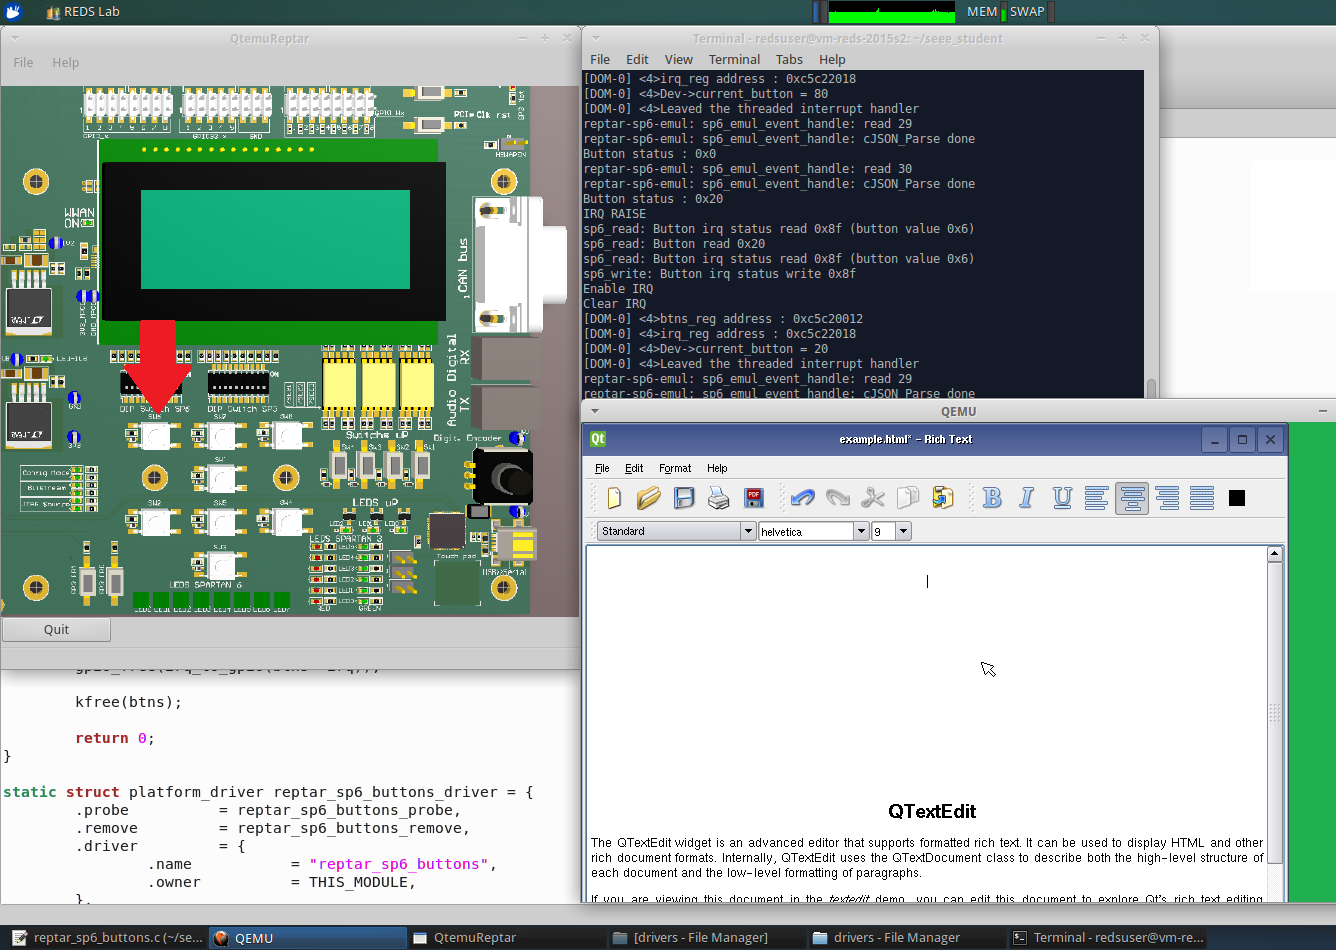
\includegraphics[width=16cm]{img/dom02.png}
		\caption{Qtrun dans Dom0}
		\label{qtrun2}
	\end{center}
\end{figure}
\begin{figure}[H]
	\begin{center}
		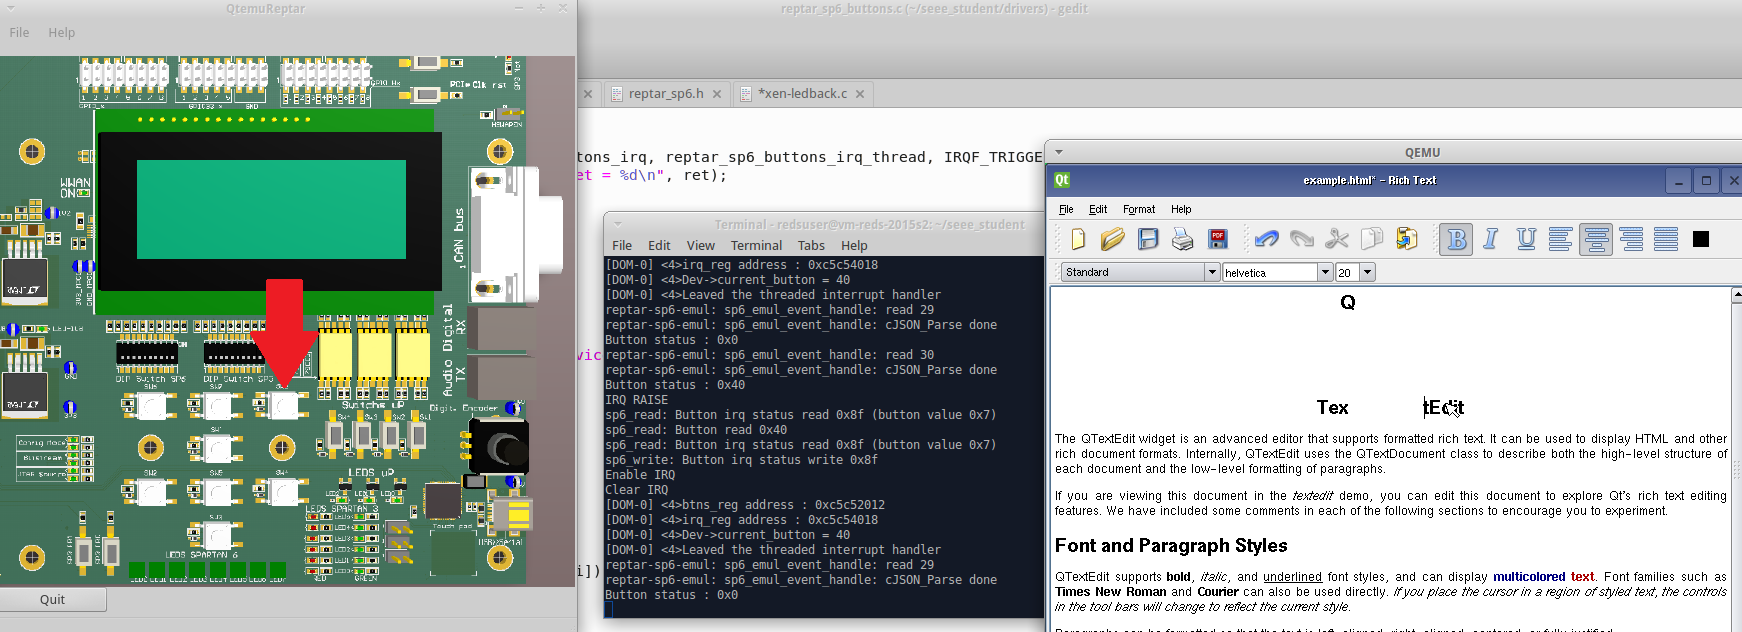
\includegraphics[width=16cm]{img/dom03.png}
		\caption{Qtrun dans DomU}
		\label{qtrun3}
	\end{center}
\end{figure}
\textbf{Réponse aux questions: }Expliquer le cheminement de l'événement input depuis l'appui sur un bouton, jusqu'au traitement applicatif.\\\\
\textbf{Travail réalisé: }Dans la première partie de cette tâche, le cheminement de l'input vers DomU est déjà expliqué. Ci-dessous est présenté le cheminement de l'événement dans Dom0
\begin{figure}[H]
	\begin{center}
		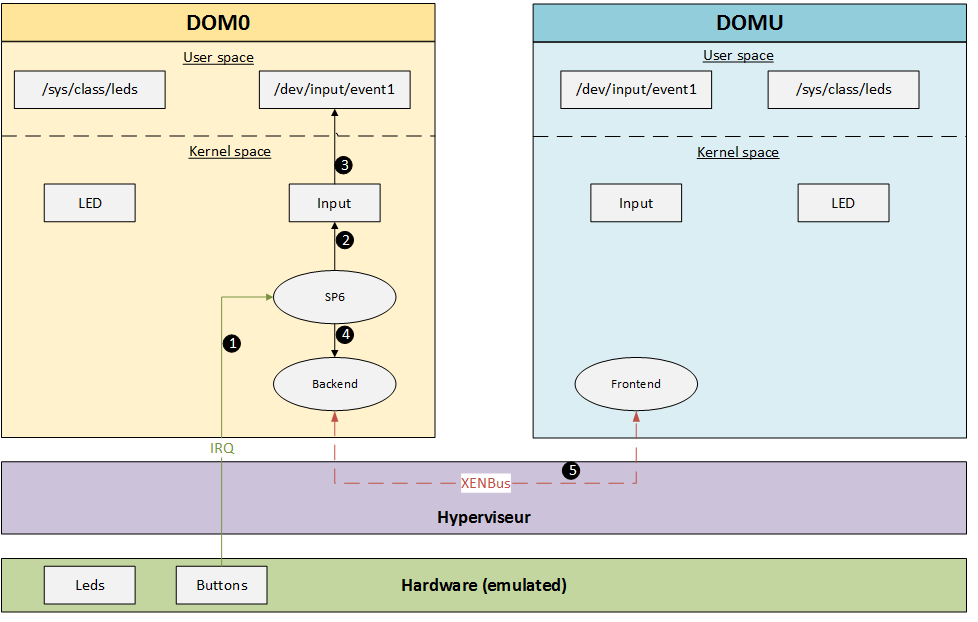
\includegraphics[width=17cm]{img/virt2.png}
		\caption{Cheminement de l'événement input}
		\label{virt2}
	\end{center}
\end{figure}
Étapes de la propagation:
\begin{enumerate}
	\item Le driver SP6 intercepte l'interruption matérielle des boutons
	\item Comme le focus est sur Dom0, l'événement est transmis au module input de Dom0
	\item L'événement se retrouve finalement en espace utilisateur dans le fichier \textit{/dev/input/event1}
\end{enumerate}
\subsection{Para-virtualisation de l'interface LED}
Nous allons maintenant nous intéresser à l’interface LED. Au terme de cet exercice, nous aurons écrit
une application, dans DomU, qui interceptera les evénements input des boutons et réagira en allumant
une LED.\\\\
\textbf{a) Donnée: }Tout d’abord, il est nécessaire de fournir une interface virtuelle LED dans DomU. Ouvrez le
fichier linux-3.4.6-domU/drivers/leds/xen-ledfront.c . Complétez le fichier pour créer les entrées
nécessaires dans /sys/class/leds et pour que les requêtes d’allumage et d’extinction des LEDs
soient propagées vers Dom0.\\\\
\textbf{Emplacement du code: }\textit{/virtualisation\_part4/xen-ledfront.c}\\\\
\textbf{Travail réalisé: }Nous nous sommes inspirés de ce qui était fait dans le driver des leds. Nous avons recréé une structure simplifiée appelée \textit{backend\_led}. L'id identifie la Led, le cdev contient le nom sous lequel elle apparaitra dans le sysfs et le callback qui sera appelé pour l'allumer/éteindre.
\begin{lstlisting}
struct backend_led {
struct led_classdev cdev;
uint8_t id;
};
\end{lstlisting}
Nous avons six Leds à piloter, nous avons donc créé une structure de six backend\_led et nous l'avons initialisée. Toutes les leds ont la même méthode de callback
\begin{lstlisting}
struct backend_led back_leds[] = {
{
.cdev.name		= "led0",
.cdev.brightness_set 	= backend_led_set,
.id			= 0
},
{
.cdev.name		= "led1",
.cdev.brightness_set 	= backend_led_set,
.id			= 1
},
...
\end{lstlisting}
Nous avons également implémenté le callback pour activer/désactiver les leds. La macro container\_of a été utilisée pour identifier avec quelle Led interagir. La macro va retourner un pointeur sur l'élément du tableau back\_leds qui est identique au paramètre de la méthode, led\_cdev.
\begin{lstlisting}
static void backend_led_set(struct led_classdev *led_cdev, enum led_brightness value)
{
	struct backend_led * led = container_of(led_cdev, struct backend_led, cdev);
	send_led_request(led->id,value);
}
\end{lstlisting}
Dans la fonction probe, il faut enregistrer chacune des six Leds comme ci-dessous pour qu'elles apparaissent dans le sysfs.
\begin{lstlisting}
/* Register the sysfs entries for the LED subsystem*/
led_classdev_register(&dev->dev, &back_leds[0].cdev);
led_classdev_register(&dev->dev, &back_leds[1].cdev);
led_classdev_register(&dev->dev, &back_leds[2].cdev);
led_classdev_register(&dev->dev, &back_leds[3].cdev);
led_classdev_register(&dev->dev, &back_leds[4].cdev);
led_classdev_register(&dev->dev, &back_leds[5].cdev);
\end{lstlisting}
La capture ci-dessous présente les différentes étapes pour compiler les changement du frontend et insérer le driver sp6 dans Dom0
\begin{lstlisting}
$ cd ~/seee_student/embeddedxen/
$ make
...
-----------------------------------------------------[ BUILDING EmbeddedXEN Hypervisor DONE ]---
$ cd ..
$ ./deploy ex
Deploying into EmbeddedXEN rootfs ...
...
Done !
$ ./stex
...
Reptar # boot
...
[DOM-U] *** Welcome on REPTAR (HEIG-VD/REDS): use root/root to log in ***
reptar login: root
Password: 
# *** Serial input -> DOMU (type 'CTRL-a' three times to switch input to Xen).
[DOM-0] <4>*** Serial input -> Xen (type 'CTRL-a' three times to switch input to DOM0).
[DOM-0] <4>*** Serial input -> DOM0 (type 'CTRL-a' three times to switch input to DOMU).

# cd
# insmod /sp6.ko
[DOM-0] <4>reptar_sp6: module starting...
[DOM-0] <4>Probing FPGA driver (device: fpga)
[DOM-0] <7>Registered led device: sp6_led0
[DOM-0] <7>Registered led device: sp6_led1
[DOM-0] <7>Registered led device: sp6_led2
[DOM-0] <7>Registered led device: sp6_led3
[DOM-0] <7>Registered led device: sp6_led4
[DOM-0] <7>Registered led device: sp6_led5
[DOM-0] <4>btns_reg address : 0xc5c60012
[DOM-0] <4>irq_reg address : 0xc5c62018
[DOM-0] <6>input: reptar_sp6_buttons as /devices/platform/fpga/reptar_sp6_buttons/input/input1
[DOM-0] <4>reptar_sp6: done.
#
\end{lstlisting}
Une fois le driver inséré, on peut retourner dans DomU. En regardant dans le \textit{/sys/class/leds}, on peut voir que les six leds sont bien présentes avec le nom qu'on leur a choisi. Chacune des leds possède également le sous-fichier brightness utilisé pour allumer/éteindre la Led.
En essayant d'écrire dans ce fichier avec la commande \textit{echo}, on ne voit pas de Led s'allumer puisque le backend n'est pas implémenté, mais on constate qu'il reçoit bien l'information correctement. En effet, dans Dom0, le backend affiche un message s'il reçoit quelque chose de la part du frontend, \textit{receive\_led\_request(led id, valeur)}
\begin{lstlisting}
# [DOM-0] <4>*** Serial input -> DOMU (type 'CTRL-a' three times to switch input to Xen).
[DOM-U] 
[DOM-U] *** Welcome on REPTAR (HEIG-VD/REDS): use root/root to log in ***
reptar login: root
[DOM-U] Password: 
[DOM-U] # cd /
# ls /sys/class/leds/
[DOM-U] led0  led1  led2  led3  led4  led5
# ls /sys/class/leds/led0
[DOM-U] brightness      device          max_brightness  subsystem       uevent
# echo 1 > /sys/class/leds/led1/brightness 
[DOM-U] # receive_led_request(1, 1)
\end{lstlisting}
\textbf{b) Donnée: }Ouvrez le fichier linux-3.0-reptar-dom0/drivers/leds/xen-ledback.c . Complétez le fichier pour que
les requêtes d’allumage et d’extinction des LEDs provenant de DomU soient traitées et effectuent
l’action désirée.\\\\
\textbf{Emplacement du code: }\textit{/virtualisation\_part4/xen-ledback.c}\\\\
\textbf{Travail réalisé: }\\
Dans la fonction probe du backend, on va faire un ioremap du registre des Leds. Il ne faut faire cette action qu'une seule fois. On a maintenant le même accès aux Leds que le driver sp6, sans avoir à communiquer avec lui pour demander l'allumage des Leds.
\begin{lstlisting}
	// Remap the /sys/class/leds to access it
	reg = ioremap(0x18000000+0x3a,2);
\end{lstlisting}
Dans la méthode \textit{receive\_led\_request}, on va simplement allumer la led voulue si brightness est plus grand que 0 ou sinon l'éteindre.
\begin{lstlisting}
	// Set the led brightness
	if(brightness)
	*reg |= 0x0001 << id;
	else
	*reg &= ~ (0x0001 << id);
\end{lstlisting}
Si l'on reprend toutes les étapes faite dans la démonstration de la partie précédente et que l'on retente d'écrire les Leds avec \textit{echo} dans DomU, on voit cette fois la Led choisie qui s'allume.
\begin{lstlisting}
# echo 1 > /sys/class/leds/led1/brightness 
[DOM-U] # receive_led_request(1, 1)
\end{lstlisting}
Voici la preuve d'allumage d'une Led. La Led 1 est bien verte, comme désiré.
\begin{figure}[H]
	\begin{center}
		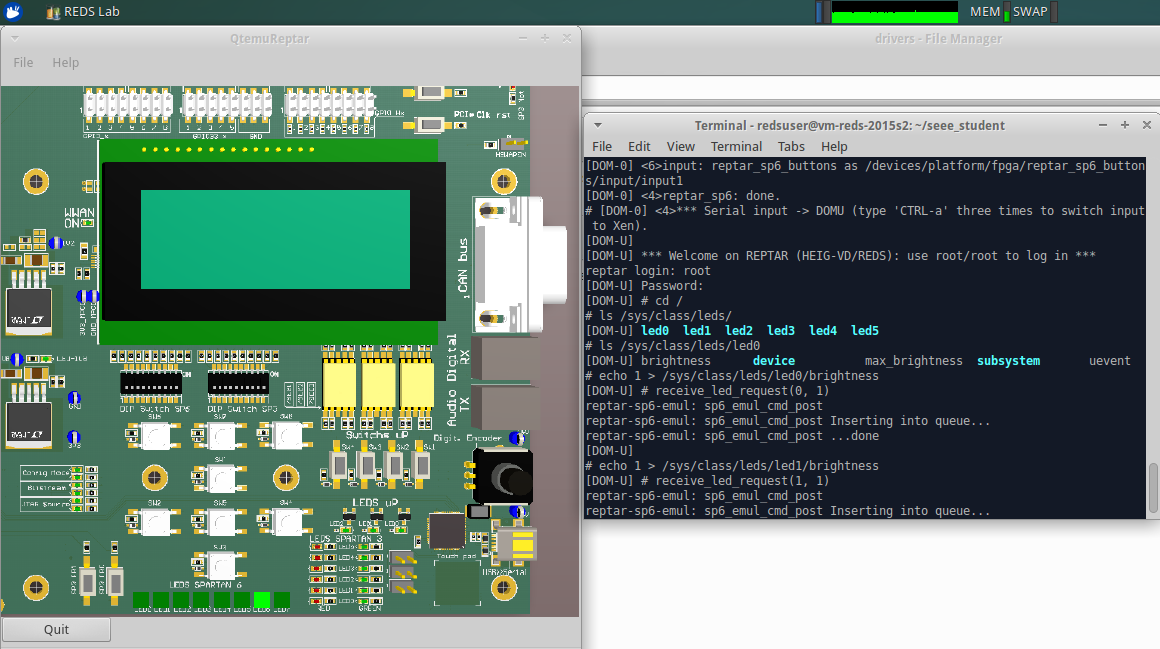
\includegraphics[width=17cm]{img/dom04.png}
		\caption{Allumage des Leds depuis DomU}
		\label{dom04}
	\end{center}
\end{figure}
\textbf{Réponse aux questions: }Vous devez maintenant être en mesure d'expliquer le cheminement depuis l’écriture de la valeur
dans l’entrée sysfs d’une LED dans DomU, jusqu’à la mise à jour du registre FPGA dédié aux LEDs
par Dom0.\\\\
\textbf{Travail réalisé: } Les deux images suivantes présentent le cheminement de l'écriture depuis le user space de DomU et dans la deuxième image, depuis Dom0.
\begin{figure}[H]
	\begin{center}
		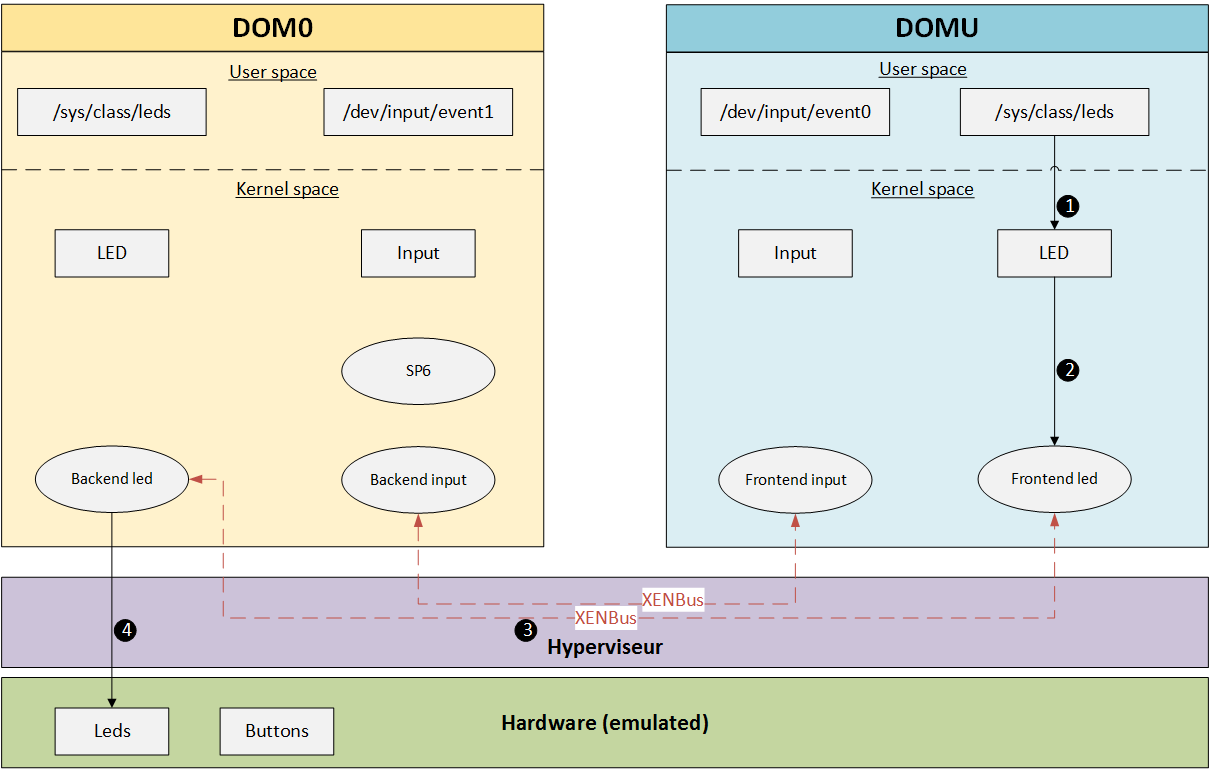
\includegraphics[width=17cm]{img/virt3.png}
		\caption{Contrôle des Leds depuis DomU}
		\label{virt3}
	\end{center}
\end{figure}
Étapes de la propagation:
\begin{enumerate}
	\item Une écriture depuis DomU dans le sysfs des Leds est transmise au module Led
	\item Le frontend led de DomU qui reçoit les callback du module Led intercepte la demande d'interaction avec les Leds.
	\item L'hyperviseur transmet l'information au travers du XenBus
	\item Le driver backend led de Dom0 reçoit le requête du frontend de DomU et va appliquer l'action correspondante directement sur les leds.
\end{enumerate}
\begin{figure}[H]
	\begin{center}
		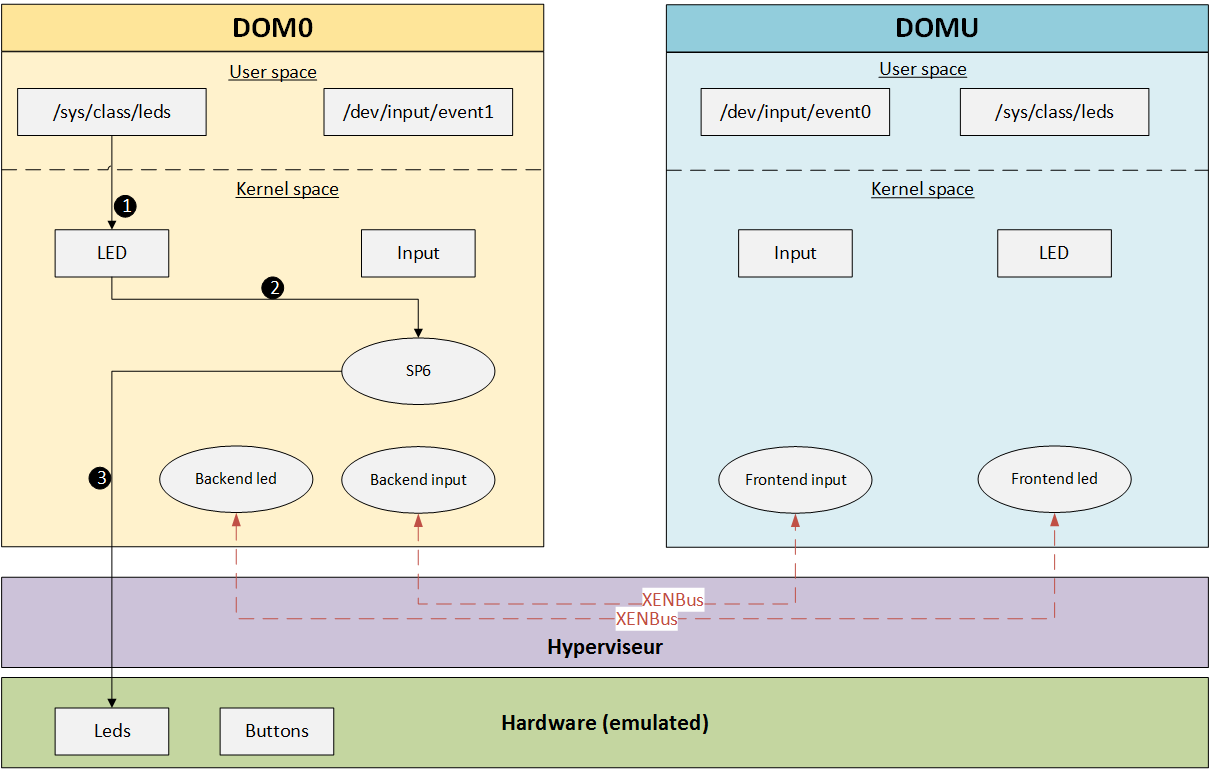
\includegraphics[width=17cm]{img/virt4.png}
		\caption{Contrôle des Leds depuis Dom0}
		\label{virt4}
	\end{center}
\end{figure}
Étapes de la propagation:
\begin{enumerate}
	\item Depuis Dom0, le chemin est plus court. L'écriture dans le sysfs des Leds est intercepté par le module led de Dom0
	\item L'événement est transmis à notre driver Sp6
	\item Le driver sp6 va appliquer l'action correspondante directement sur les Leds.\\
\end{enumerate}
\textbf{c) Donnée: }Écrivez une application qui doit respecter les critères suivants :
\begin{enumerate}
	\item Un appui sur le bouton numéro 2 (gauche) allume la LED 2, un appui sur le bouton numéro 5 (centre)
	allume la LED 1 et un appui sur le bouton numéro 4 (droite) allume la LED 0. Un appui sur le
	bouton numéro 3 (bas) éteint les LEDs.
	\item L’application fait du polling sur /dev/input/event0 pour détecter l’appui sur un bouton. Elle
	doit décoder la valeur de la touche pour identifier le bouton.
	\item L’application utilise les entrées sysfs liées au sous-système LED.
\end{enumerate}
Testez sur l’émulateur et sur la plate-forme réelle.\\\\
\textbf{Emplacement du code:}\\\textit{/virtualisation\_part4/test\_input.c}\\
\textit{/virtualisation\_part4/Makefile}\\
\textit{/virtualisation\_part4/reptar\_sp6.c}\\\\

\textbf{Travail réalisé: }
L'application se compose, globalement, d'une boucle infinie qui va poller le fichier \textit{/dev/input/event0}. Celui-ci renvoie, sous la forme d'une structure de type \textit{input\_event} les événements qui se sont produits au niveau des boutons. On obtient ainsi, après avoir contrôlé la valeur (1 si la touche a été enfonçée et 0 si relâchée) et le type (devant correspondre à \textit{EV\_KEY}), le code, qui désigne quel bouton a été appuyé.\\
Trois fichiers sont importants pour le contrôle des leds. Leur nom ressemble à \textit{/sys/class/leds/ledx/brightness}. Ceci veut dire qu'elles ont été enregistrées dans le système de fichier \textit{/sysfs} par un driver auparavant. Lorsqu'on écrit un \textit{1} dans ces fichiers, les leds correspondantes s'allument. Et pour un \textit{0} elles s'éteignent. Dans cette application, une fonction est utilisée pour manipuler les leds, avec en paramètre le numéro de la led et son état, \textit{0} ou \textit{1}. Le fichier est ouvert, on y écrit la valeur, et ensuite, on le referme. \\
Le makefile présent dans le dossier des drivers a été modifié pour compiler cette petite application. Les deux lignes suivantes ont été modifiées:
\begin{lstlisting}
	all: kernel buttons_test usertest test_input
	...
	test_input: test_input.c
		$(CC) -marm -I$(KDIR) -static test_input.c -o test_input
\end{lstlisting}
Une modification a aussi été apportée à \textit{Qemu} et en particulier à notre fichier \textit{reptar\_sp6.c}. En effet, l'application crashait dès que nous pressions sur un bouton. Cela était du à la construction et au remplissage des paquets JSON en dehors des zones où nous en avions effectivement besoin.

\begin{lstlisting}
	cJSON *root;

	switch(offset)
	{
	case SP6_LED:
		if(size == 2)
		{
			root = cJSON_CreateObject();
			cJSON_AddStringToObject(root,"perif","led");
			//printf ("sp6_write: Led write 0x%x\n",value);
			led_register_value = (uint16_t) value;
			//Create JSON response
			cJSON_AddNumberToObject(root,"value",led_register_value);
			sp6_emul_cmd_post(root);
		}
\end{lstlisting}
On instançiait le paquet JSON sans savoir si nous allions effectivement l'utiliser. Le code d'allocation se trouvait au dehors du \textit{switch case}. Le fait d'instancier l'objet uniquement lors de son utilisation, c-à-d dans le \textit{case} et dans le \textit{if} a résolu le problème. La fonction \textit{sp6\_emul\_cmd\_post(root);} poste le paquet JSON et s'occupe de désallouer l'espace grâce au pointeur passé en argument. L'ancien code permettait d'allouer de l'espace sans pour autant le désallouer automatiquement. 

\textbf{Remarque: }Pour pouvoir insérer notre application dans le rootfs de DomU, nous avons dû télécharger une nouvelle version du script \textit{deploy ex}. Un répertoire domu est créé dans notre workspace. Il faut absolument placer l'exécutable de l'application dans ce dossier pour qu'il soit ensuite visible dans DomU.\\\\
Voici les différents tests effectués avec l'application. Une fois le driver sp6 inséré dans Dom0. Il faut aller lancer notre application test\_input dans DomU. Il est ensuite important d'appuyer sur le bouton en haut à droite pour changer le focus sur DomU, sinon les événements des boutons ne seront pas transmis et resteront dans Dom0.
L'application remplit tous les critères demandés.
\begin{lstlisting}
[DOM-U] *** Welcome on REPTAR (HEIG-VD/REDS): use root/root to log in ***
reptar login: root
Password: 
# *** Serial input -> DOMU (type 'CTRL-a' three times to switch input to Xen).
[DOM-0] <4>*** Serial input -> Xen (type 'CTRL-a' three times to switch input to DOM0).
[DOM-0] <4>*** Serial input -> DOM0 (type 'CTRL-a' three times to switch input to DOMU).

# cd
# insmod /sp6.ko 
[DOM-0] <4>reptar_sp6: module starting...
[DOM-0] <4>Probing FPGA driver (device: fpga)
[DOM-0] <7>Registered led device: sp6_led0
[DOM-0] <7>Registered led device: sp6_led1
[DOM-0] <7>Registered led device: sp6_led2
[DOM-0] <7>Registered led device: sp6_led3
[DOM-0] <7>Registered led device: sp6_led4
[DOM-0] <7>Registered led device: sp6_led5
[DOM-0] <4>btns_reg address : 0xc5c20012
[DOM-0] <4>irq_reg address : 0xc5c22018
[DOM-0] <6>input: reptar_sp6_buttons as /devices/platform/fpga/reptar_sp6_buttons/input/input1
[DOM-0] <4>reptar_sp6: done.
# [DOM-0] <4>*** Serial input -> DOMU (type 'CTRL-a' three times to switch input to Xen).
[DOM-U] 
[DOM-U] *** Welcome on REPTAR (HEIG-VD/REDS): use root/root to log in ***
reptar login: root
[DOM-U] Password: 
[DOM-U] # cd /
# ./test_input 
\end{lstlisting}
\begin{figure}[H]
	\begin{center}
		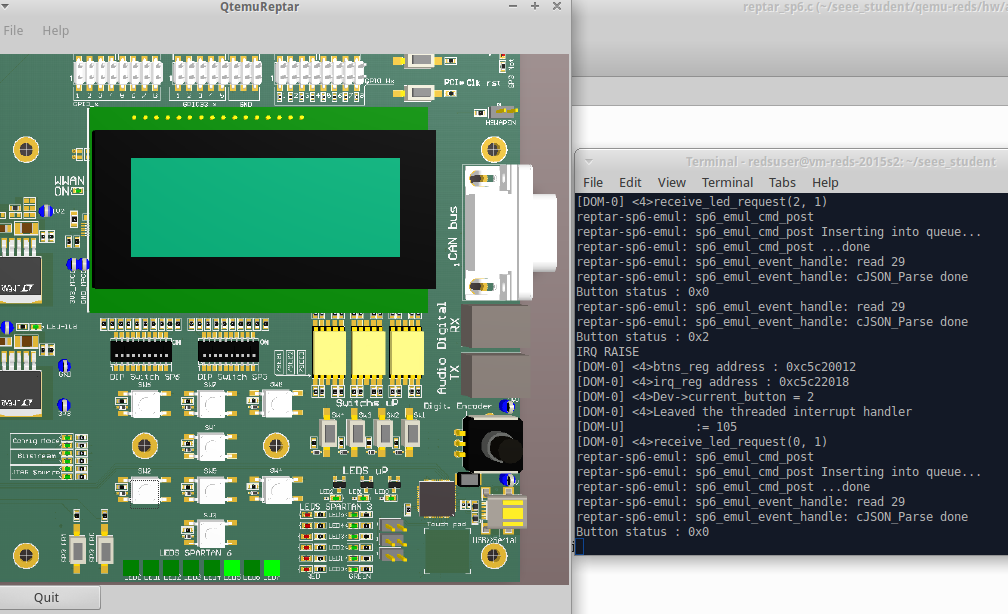
\includegraphics[width=17cm]{img/dom05.png}
		\caption{Tests de l'application dans DomU}
		\label{dom05}
	\end{center}
\end{figure}
\textbf{Remarque: }Nous n'avons malheureusement pas eu le temps de tester notre application sur la plateforme réelle, mais nous l'avons tout de même entièrement validée avec l'émulateur.\\\\
\textbf{d) Donnée: }Nous souhaitons maintenant nous passer des traitements dans l’user space. Proposez une solution
dans le kernel space qui ne fait intervenir aucune interaction avec l’user space. Implémentez-la.
Le comportement doit être le même qu’en c). Testez sur l’émulateur et la plate-forme réelle.\\\\
\textbf{Emplacement du code: }\\\textit{/virtualisation\_part4/xen-kbdfront.c}\\
\textit{/virtualisation\_part4/xen-ledfront.c}\\\\
\newpage
\textbf{Travail réalisé: }Voici la solution que nous voulons implémenter
\begin{figure}[H]
	\begin{center}
		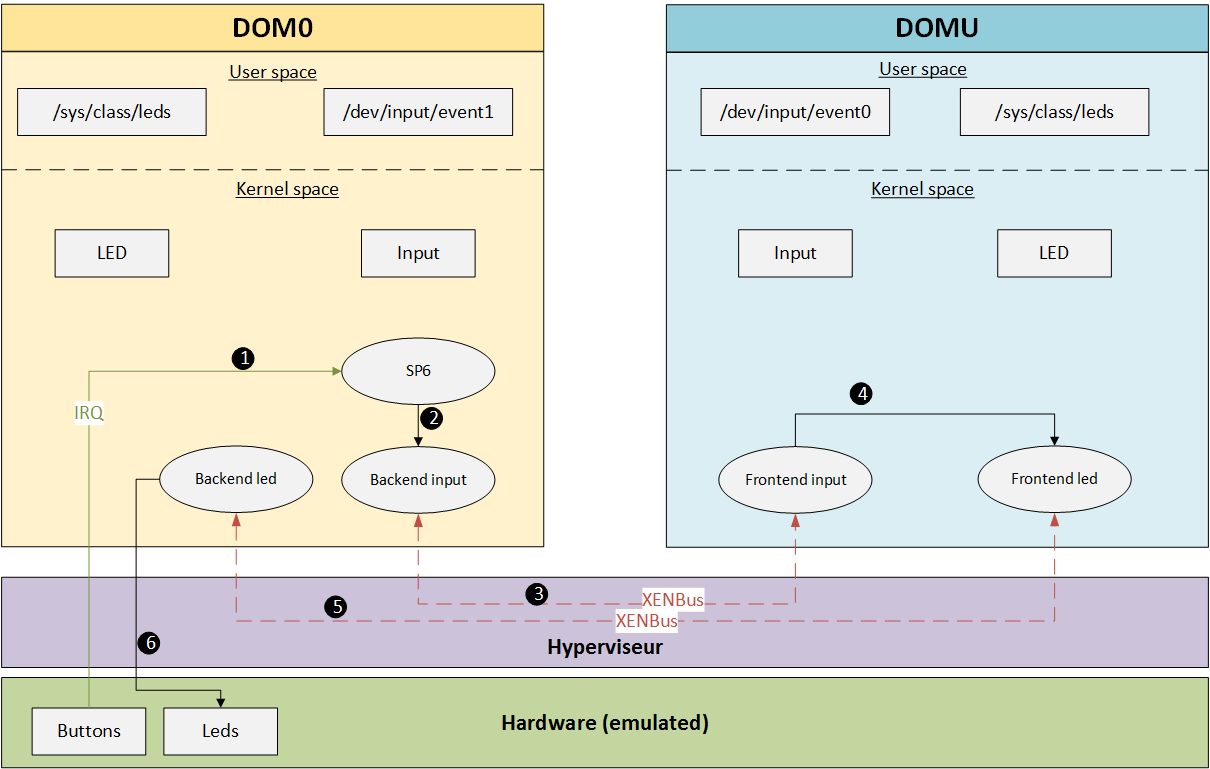
\includegraphics[width=17cm]{img/virt5.png}
		\caption{Traitement des événements sans interactions avec le User space}
		\label{virt5}
	\end{center}
\end{figure}
Étapes de la propagation:
\begin{enumerate}
	\item L'interruption matérielle est interceptée par notre driver SP6 qui est présent uniquement dans Dom0
	\item Si le focus est placé sur DomU, l'événement est propagé au driver backend input. Notre driver SP6 s'est préalablement enregistré auprès du backend.
	\item L'hyperviseur transmet l'information au travers du XenBus
	\item Le driver frontend input de DomU reçoit l'input event. Il analyse quel bouton a été pressé et quelle Led allumer. Il appelle la méthode send\_led\_request() du frontend led pour envoyer une requête d'allumage de Led vers Dom0
	\item La demande est ensuite transmise sur le XenBus
	\item Le backend led driver de Dom0 reçoit la requête et applique le traitement correspondant directement sur les leds.
\end{enumerate}
Avec ce cheminement, on se passe complètement de l'interaction avec le user space dans DomU et on peut avoir les mêmes résultats que l'application du point c.\\\\
Nous avons modifié le fichier \textit{xen-kbdfront.c} pour appliquer directement le traitement des boutons sur les Leds.\\
Afin de pouvoir appeler la méthode send\_led\_request du frontend led, nous avons dû la déclarer externe dans ce fichier.
\begin{lstlisting}
extern void send_led_request(int id, int brightness);
\end{lstlisting}
Il a fallu également changer le type de la méthode en non static dans le fichier \textit{xen-ledfront.c}. Si on ne le fait pas, on ne peut pas l'appeler depuis l'extérieur.\\\\
L'étape suivante est d'appliquer le même code que dans l'application développée en c lors de la réception d'un input event. Cela est fait dans la méthode \textit{input\_handler}. Comme nous avons enregistrer un driver de type GPIOKEY dans le driver sp6, nous avons appliqué le traitement lorsque l'événement est de type XENKBD\_TYPE\_KEY.
\begin{lstlisting}
case XENKBD_TYPE_KEY:
	dev = NULL;
	if (test_bit(event->key.keycode, info->kbd->keybit))
		dev = info->kbd;
	if (test_bit(event->key.keycode, info->ptr->keybit))
		dev = info->ptr;
	if (dev)
	{
	//input_report_key(dev, event->key.keycode,event->key.pressed);
		if(event->key.pressed == 1)
		{
			switch (event->key.keycode) 
			{
				case RIGHT_BUT:
					send_led_request(0,1);
					break;
				case CENTER_BUT:
					send_led_request(1,1);
					break;
				case LEFT_BUT:
					send_led_request(2,1);
					break;
				case BOTTOM_BUT:
					for(i = 0; i < LED_NUM; i++)
						send_led_request(i,0);
					break;
				default:
					break;
			}
		}
	}
\end{lstlisting}
Pour tester ces nouvelles fonctionnalité, il suffit de recompiler les fichiers que nous avons modifier et de lancer Qemu. La dernière étape est d'insérer le driver dans Dom0.
\begin{lstlisting}
# cd
# insmod /sp6.ko 
[DOM-0] <4>reptar_sp6: module starting...
[DOM-0] <4>Probing FPGA driver (device: fpga)
[DOM-0] <7>Registered led device: sp6_led0
[DOM-0] <7>Registered led device: sp6_led1
[DOM-0] <7>Registered led device: sp6_led2
[DOM-0] <7>Registered led device: sp6_led3
[DOM-0] <7>Registered led device: sp6_led4
[DOM-0] <7>Registered led device: sp6_led5
[DOM-0] <4>btns_reg address : 0xc5c34012
[DOM-0] <4>irq_reg address : 0xc5c36018
[DOM-0] <6>input: reptar_sp6_buttons as /devices/platform/fpga/reptar_sp6_buttons/input/input1
[DOM-0] <4>reptar_sp6: done.
# 
\end{lstlisting}
Une fois le driver inséré, si le focus est sur Dom0 et que l'on appuie sur les boutons, aucune Led ne s'allume. Si on place le focus sur DomU, l'appui sur les boutons définis allument ou éteignent les Leds.
\begin{figure}[H]
	\begin{center}
		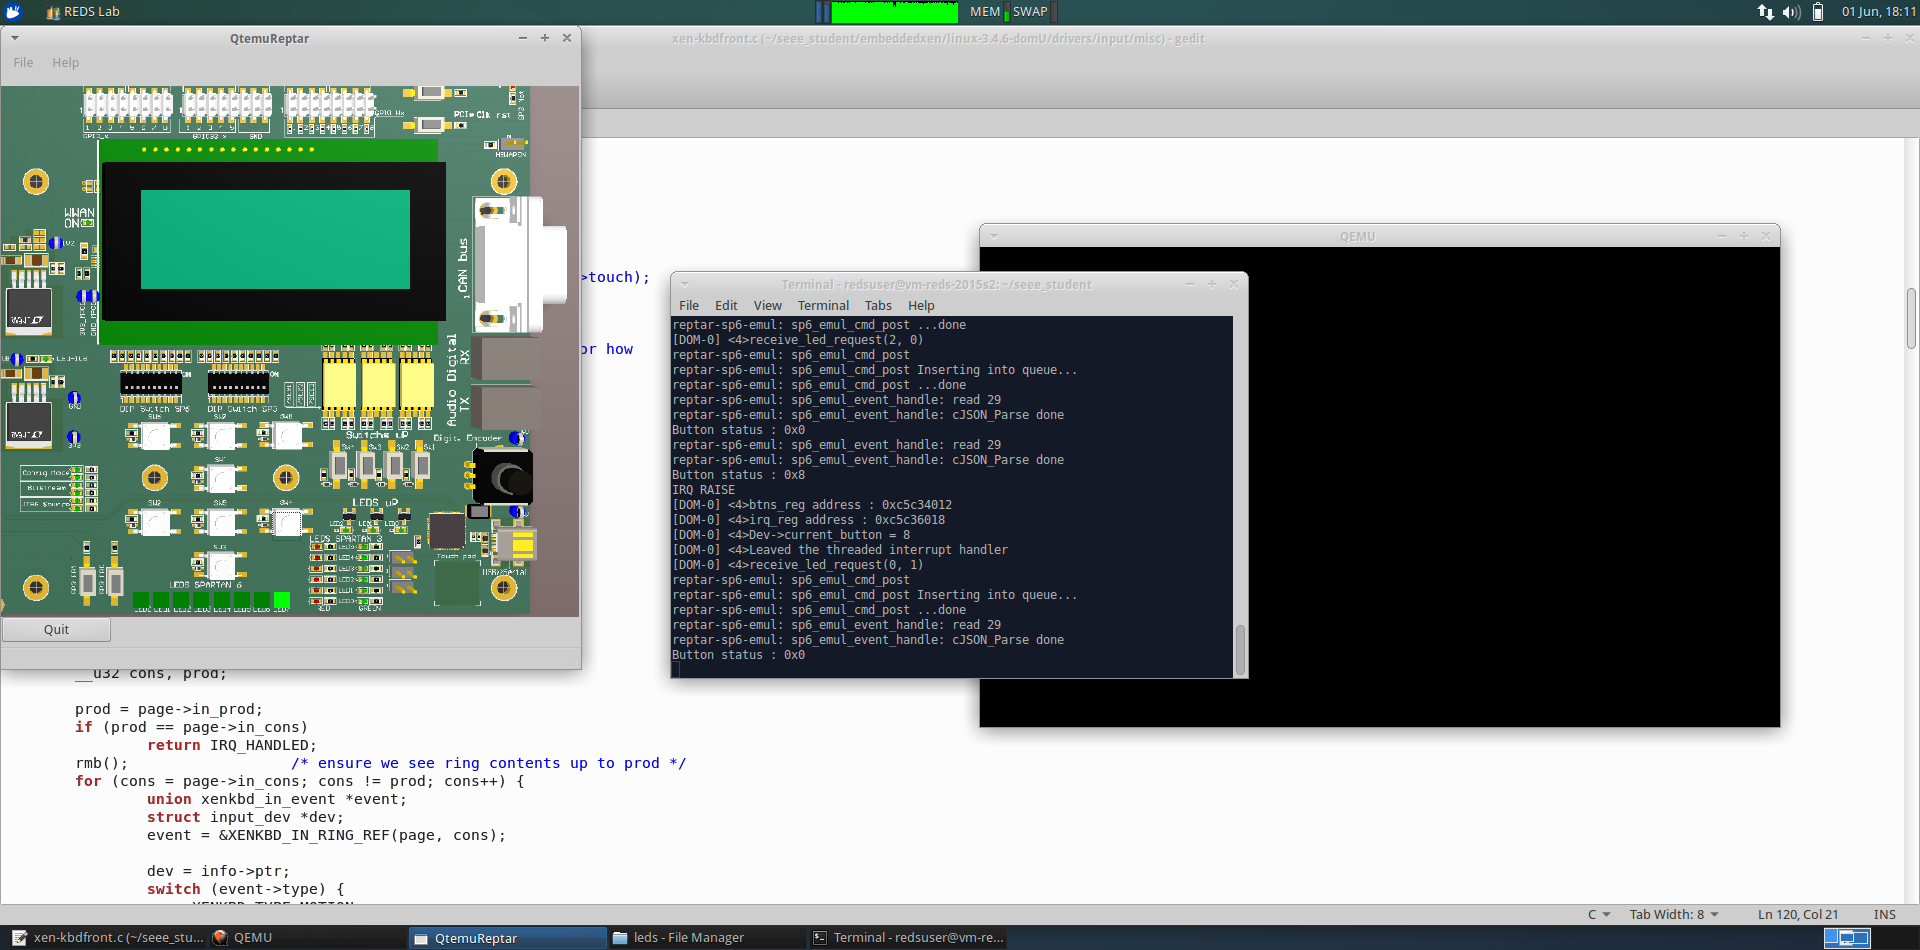
\includegraphics[width=17cm]{img/dom06.png}
		\caption{Allumage des leds sans interaction avec le user space}
		\label{dom06}
	\end{center}
\end{figure}
\textbf{Remarque: }Nous n'avons malheureusement pas eu le temps de tester cette partie sur la plateforme réelle, mais nous avons pu valider son fonctionnement avec l'émulateur.